\chapter{Descrição do problema e do sistema proposto}
Como comentado, o presente trabalho é motivado pela carência de conjuntos de dados abertos e robustos de imagens de doenças em folhas de plantas, que possibilitem o desenvolvimento de modelos de visão computacional com aplicabilidade prática no cotidiano dos produtores rurais.

\subsection{Considerações}
Para que um conjunto de dados com essa potencialidade seja desenvolvido, é preciso levar em conta algumas considerações importantes. Dentre elas, podemos destacar as seguintes:

\begin{enumerate}
{\bf \item  Volume considerável de dados:}

No contexto de \emph{deep learning}, modelos de visão computacional já se provaram muito efetivos. Contudo, é consenso que grandes quantidades de dados são necessárias para evitar \emph{overfitting}.

A ideia geral de sistemas supervisionados de \emph{machine learning}, é que, utilizando de algoritmos de otimização de uma função de perda --- que quantifica a performance do modelo atual --- os modelos em treinamento aprendam a reproduzir a função representada pelo conjunto de dados. Em que os dados de entrada são as variáveis independentes (no caso, imagens) e os rótulos são as variáveis dependentes \citep{Yaser:2012}. 

Nesse caso, quando não temos uma grande quantidade de dados, os modelos de aprendizado profundo (\emph{deeplearning}) têm a capacidade de aprender uma função que reproduz perfeitamente o conjunto de treinamento, é como se o modelo ``decorasse'' os dados ao invés de relacionar características importantes neles para chegar a respostas pertinentes \citep{Yaser:2012, Shorten2019A}. 

Por isso, esses sistemas necessitam de grandes quantidades de dados para funcionarem de maneira satisfatória \citep{Shorten2019A}. Então, para construir um conjunto de dados de qualidade para detecção de doenças em folhas de plantas, é importante que ele tenha um volume considerável.

{\bf \item Os dados devem contemplar a variabilidade dos casos de uso real da tecnologia:}
Para que modelos de \emph{machine learning} sejam capazes de generalizar bem, é necessário que, o conjunto de dados com os quais são treinados representem bem a diversidade dos dados que estarão presentes no cotidiano de uso da tecnologia resultante. Isso ocorre porque, quando os dados presentes nos casos de uso real da ferramenta forem muito diferentes dos dados de treinamento, o modelo simplesmente não terá tido contato com dados de tal natureza e, portanto performará pobremente. 

Um exemplo claro disso é o tipo de imagens presentes no \emph{dataset PlantVillage}. Essas imagens, com aspecto de ``laboratório'' (folhas retiradas das plantas e dispostas em superfícies planas e de cor sólida) certamente são diferentes das imagens disponíveis no contexto do campo: características como planos de fundo com alta variabilidade (plantas, paisagens, etc.) e folhas ainda presas nos galhos são exemplos disso.

{\bf \item Os dados devem passar por uma curadoria especializada:}

No domínio de detecção de doenças em plantas, uma avaliação de especialistas sobre os dados, para produzir rótulos corretos é de suma importância. Isso ocorre pois muitas vezes, não é fácil diferenciar as doenças entre si, devido à elevada similaridade entre sintomas e pelo simples fato dessa identificação não ser conhecimento ``comum''.

{\bf \item Não deve haver duplicatas ou ``quase-duplicatas'' nos dados:}

A presença de dados duplicados, ou ``quase-duplicados'' em conjuntos de dados é maléfica para o treinamento de modelos de \emph{machine learning}. Isso ocorre pois durante a etapa de treinamento, o modelo pode decorar padrões presentes nas imagens duplicadas e isso implica no comprometimento da performance dos modelos ao se deparar com dados inéditos \citep{Barz2019Do}. 

Além disso, a inclusão desses dados ``repetidos'' pode levar a uma similaridade elevada entre os conjuntos de treino e teste do \emph{dataset}. Nesse caso, como a avaliação do modelo é realizada com base no conjunto de teste, a presença de dados muito semelhantes pode artificialmente inflar as métricas de desempenho, resultando em uma avaliação irreal das capacidades do modelo e na pior capacidade de generalização no momento de implantação do modelo em campo \citep{Barz2019Do}.

\end{enumerate}


\subsection{Solução proposta}
Com o levantamento dessas considerações, formulamos uma abordagem de construção colaborativa de conjuntos de dados para detecção de doenças de plantas que se propõe a ser uma possível solução para a escassez de \emph{datasets} robustos, volumosos, confiáveis e abertos nesse domínio.

\subsubsection{Redução do Escopo}
Para o desenvolvimento dessa solução, primeiramente reduzimos o escopo das tarefas propostas por grandes \emph{datasets} desse domínio \citep{Yao2023}. Tanto o \emph{PlantDoc} (um \emph{dataset} alternativo ao \emph{PlantVillage}, que oferece imagens sem a característica de imagens de ``laboratório'') quanto o próprio \emph{PlantVillage}, por exemplo, têm em suas classes o seguinte formato:
\begin{center}
    \texttt{(<espécie> : <condição>)}
\end{center}
Ou seja, além de identificar a doença que afeta a planta, o modelo também tem a tarefa de identificar a espécie da planta em questão. Na realidade, para o caso de uso abordado nesse trabalho (detecção de doenças em plantas) é esperado que o agricultor saiba, no mínimo, a espécie da planta que está cultivando. Desse modo, decidimos simplificar a tarefa para a {\bf detecção de doenças nas folhas de tomate}.

A escolha dessa cultura na redução do escopo do trabalho se deu pelo fato da hortaliça ser uma das mais consumidas no mundo e da tomaticultura ser de imensa importância no setor da agricultura brasileira, sendo uma das principais fontes de emprego e renda da produção agrícola e tendo um valor de produção bruto superior a 12,4 bilhões de reais em 2022, de acordo com dados do IBGE e matéria publicada no portal Revista Rural \footnote{\url{https://www.revistarural.com.br/2022/10/14/tecnologias-impulsionam-producao-nacional-do-tomate/}}.

\subsection{\emph{TomatoHealth}}
Desse modo, a ideia da solução proposta é implementar uma plataforma chamada \emph{TomatoHealth} que oferece a funcionalidade de detecção de doenças em folhas de tomate por meio de uma aplicação \emph{web}. Por meio dessa aplicação, os usuários podem submeter imagens das folhas de suas plantas e a aplicação retorna uma resposta sobre as doenças detectadas.

Para que isso ofereça uma possível solução para a escassez de conjuntos de dados robustos na tarefa de detecção de doenças em plantas, as imagens enviadas pelos usuários passam a fazer parte de um banco de dados. 

Então, a partir desse repositório de imagens enviadas pelos usuários, uma outra frente de atuação da plataforma permite que, para cada imagem armazenada no banco de dados, usuários privilegiados (especialistas do domínio) façam revisões da inferência efetuada pelo modelo de detecção de doenças. 

Depois dessa revisão, as imagens revisadas podem passar a integrar o conjunto de dados usado para a tarefa de detecção de doenças em folhas de tomate, fechando um ciclo de atualização contínua do conjunto de dados e melhorando, iterativamente, a robustez do conjunto de dados original.

É importante destacar que a solução implementada por essa primeira versão do \emph{TomatoHealth} aborda de maneira efetiva as seguintes considerações feitas sobre o problema tratado nesse trabalho de formatura supervisionado:

\begin{enumerate}
{\bf \item  Volume considerável de dados:} pois iterativamente, o volume do conjunto de dados é aumentado com imagens que passaram pelo crivo de especialistas;

{\bf \item Os dados contemplam a variabilidade dos casos de uso real da tecnologia:} pois as imagens que têm a possibilidade de passar a integrar o conjunto de dados são tiradas justamente do contexto de aplicação real da tecnologia;

{\bf \item Os dados passam por uma curadoria especializada:} pois a presença da figura dos especialistas atua na revisão e curadoria de todas as imagens que passam a fazer parte do conjunto de dados;

\end{enumerate}

Note que a consideração 

\begin{enumerate}
    \setcounter{enumi}{3}
    {\bf \item Não deve haver duplicatas ou ``quase-duplicatas'' nos dados}
\end{enumerate}

Não foi abordada por essa primeira versão de implementação do \emph{TomatoHealth}. Contudo, já planejamos a integração de algoritmos que façam busca por imagens semelhantes no conjunto de dados existente e as exiba para o especialista que está fazendo a revisão.

\begin{figure}
    \centering
    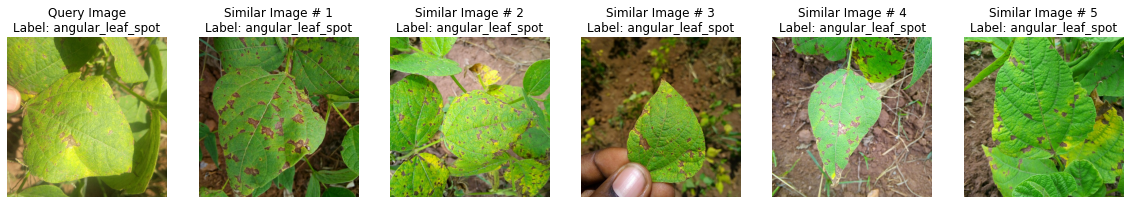
\includegraphics[width=1\linewidth]{images/results_one.png}
    \caption{\label{fig:similaridade}Exemplos de resultados do algoritmo de busca por imagens com base em similaridade. (extraído de \url{https://huggingface.co/blog/image-similarity}).}
\end{figure}

Caso a imagem que está sendo revisada apresente um grau de semelhança elevada com outras imagens que já fazem parte do conjunto de dados, o especialista terá a opção de descartar a amostra em questão. Essa funcionalidade, que fará com que a solução proposta contemple todas as considerações feitas no trabalho será melhor descrita na seção ~\ref{sec:próximos passos}.

\subsection{{Detalhes ``abstratos'' sobre o sistema} \label{sec:abst-det}}

Nessa seção, iremos descrever as capacidades esperadas do sistema desenvolvido sem detalhes de implementação.

\subsubsection{{Storyboard do sistema}}

Uma ótima forma de começar o desenvolvimento de um sistema é demonstrar seus casos de uso e aplicações no mundo real por meio de um \textit{Storyboard}. Uma técnica muito empregada por estúdios de animação, pois produzir desenhos para cada quadro de uma animação é uma tarefa demorada, e desenhar um quadro que não será usado é um desperdício (similar ao desenvolvimento de código). Além de ser rápido de esboçar, o \textit{Storyboard} permite demonstrar informações sobre um sistema que seria dificilmente explicado por texto, e também transmite informações essenciais de um sistema: usuários, contexto, sequência de tarefas de seu sistema e como seu sistema traz satisfação \citep{klemmer2016}. Sendo assim, a Figura \ref{fig:storyboard} demonstra o \textit{Storyboard} feito para o \emph{TomatoHealth}.

Na Figura \ref{fig:storyboard}, enumeramos as ações dos quadrinhos:

\begin{enumerate}
    \item Um tomateiro doente
    \item Um fazendeiro encontra seu tomateiro doente
    \item Ele tira uma foto da sua folha
    \item Ele fica alegre em descobrir a doença e como cuidar de seu tomateiro, com a ajuda de uma Inteligência Artificial
    \item A imagem tirada pelo fazendeiro é salva num banco de dados abertos
    \item Um especialista analisa as imagens salvas
    \item As imagens analisadas por um especialista são usadas para treinar a Inteligência Artificial
\end{enumerate}

\begin{figure}[ht]
    \centering
    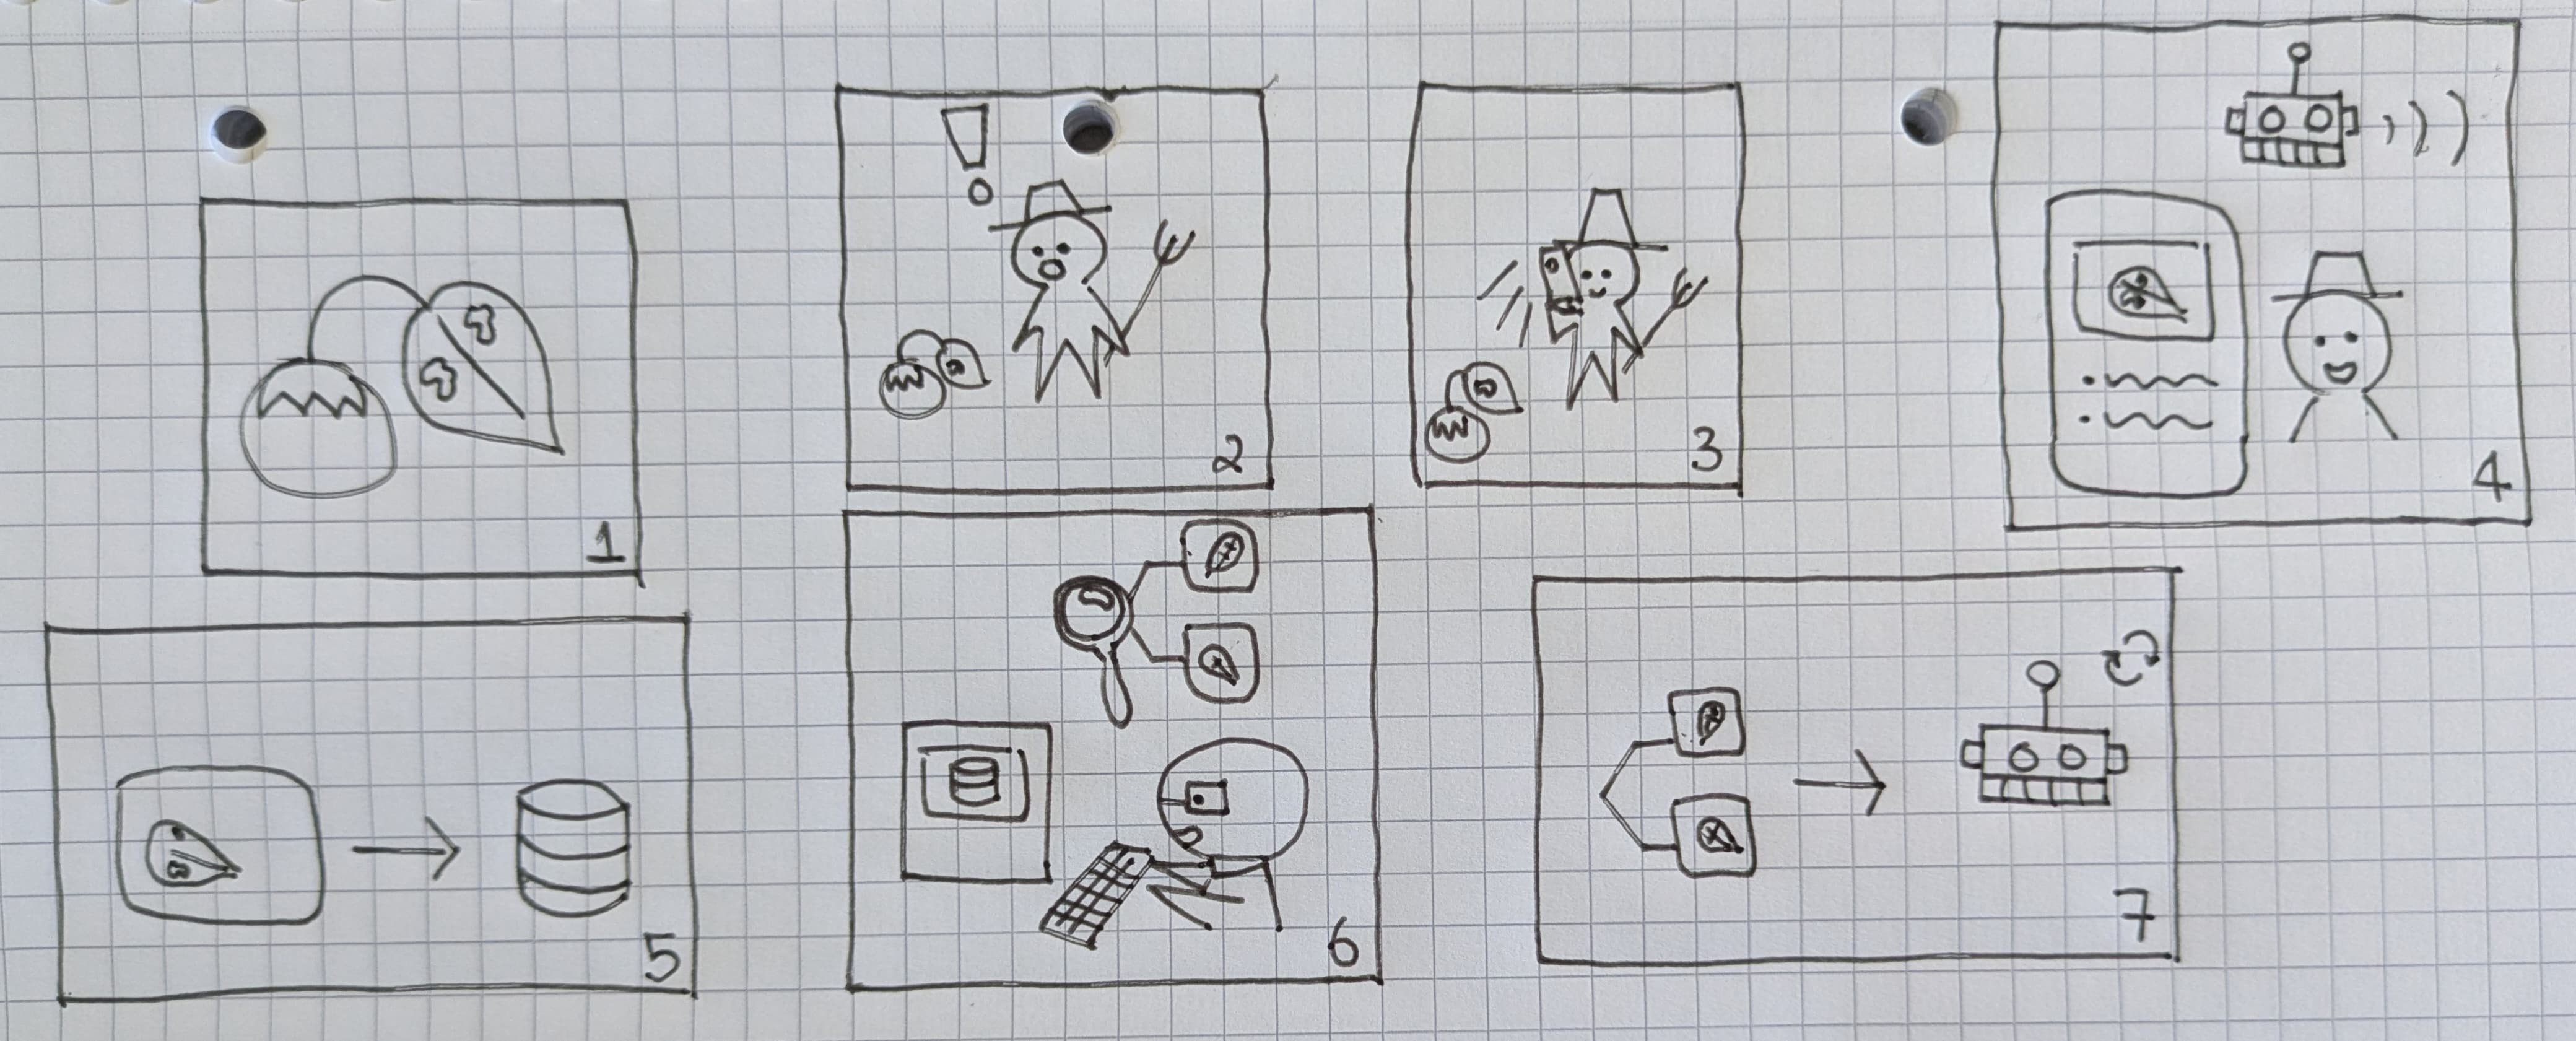
\includegraphics[width=\textwidth]{images/storyboard.jpg}
    \caption{Storyboard do desenvolvimento do sistema}
    \label{fig:storyboard}
\end{figure}

\subsubsection{{Descrição geral sobre o sistema}}

Já tendo uma breve noção sobre a atuação do \emph{TomatoHealth} por nosso \textit{Storyboard}, também é importante descrever o sistema de maneira geral, para comentar sua pertinência aos assuntos tratados nesse trabalho, e destacar como ele se relaciona ao problema.

As próximas seções separam os componentes do sistema do \emph{TomatoHealth}, para que a Seção \ref{sec:implementacao_sistema} os detalhe de maneira técnica.

\subsubsubsection{{Interface do Usuário Geral} \label{sec:abst-geral}}

Nossa interface web deve permitir ao usuário geral:

\begin{itemize}
    \item entender o papel da ferramenta
    \item tirar ou escolher uma foto de folha de tomate
    \item enviar essa foto para análise
    \item receber um \textit{feedback} sobre a saúde de seu tomateiro
\end{itemize}

Uma parte importante dessa interface é estimular o usuário a tirar uma foto de sua folha a partir de seu celular, para que essas imagens quando armazenadas e classificadas sirvam de dados em casos de usos reais em nosso \textit{dataset}.

Com esse objetivo em mente, priorizamos o desenvolvimento \textit{Mobile-first}, e permitimos o usuário a acessar a câmera de seu celular, assim como o instruímos de como tirar uma foto adequada, tanto para um \textit{feedback} quanto um dado melhor em nosso \textit{dataset}.

\subsubsubsection{{Interface do Usuário Especialista} \label{sec:abst-esp}}

Na interface do usuário especialista, ele deve ser capaz de:

\begin{itemize}
    \item autenticar com seu e-mail e sua senha
    \item ver as imagens tiradas por usuários comuns
    \item demarcar na imagem as diferentes classes que uma folha de tomate pode ter
\end{itemize}

Com isso, as imagens ficam com suas classes demarcadas por um quadrado, e inseridas em nosso banco de dados, para retreinamento do nosso modelo. 

\subsubsubsection{{\emph{back-end}}\label{sec:back-end-intro}}

Nosso \emph{Back-end} deve comportar:

\begin{itemize}
    \item a criação de usuários especialistas
    \item um banco de dados com as imagens enviadas por usuários comuns e as imagens a serem usadas no modelo de detecção
    \item o treinamento do modelo
    \item um servidor que recebe uma imagem, realiza a detecção, e faz uma chamada para uma \emph{LLM} recomendar cuidados a serem feitos com o tomateiro de acordo com as classes detectadas
    \item a inserção de imagens enviadas por usuários comuns e de imagens anotadas por especialistas no banco de dados
\end{itemize}

Dessa forma, o sistema faz o treinamento do modelo de maneira periódica com dados revisados por especialistas, e retorna um \textit{feedback} com as detecções do modelo a um usuário comum.

\subsection{{Sistemas similares -- detecção de doenças e sistemas colaborativos}}

Ao pesquisar por \textit{"plant diagnosis"} na \textit{Google Play} \footnote{\url{https://play.google.com/store/apps/}}, encontramos dezenas de aplicativos capazes de identificar culturas e/ou doenças por meio de fotos. Um dos mais populares, com mais de $10$ milhões de downloads, é o \textit{Plantix} \footnote{\url{https://plantix.net/pt/}}.

Ademais, na pesquisa por sistemas no âmbito de ciência colaborativa, encontramos duas referências semelhantes quanto a nossa proposta de sistema por compartilharem fotos fornecidas por usuários para a utilização em pesquisa, são elas: \textit{iNaturalist} \footnote{\url{https://www.inaturalist.org/}} e \textit{Zooniverse} \footnote{\url{https://www.zooniverse.org/}}.

\subsubsection{{\textit{Plantix}}}

Segundo sua página, o aplicativo tem o mesmo propósito de nosso \textit{TomatoHealth}, mas para diversas culturas. Entretanto, além do sistema identificar doenças e propor tratamentos, ele fornece ao usuário o contato com especialistas para sanar dúvidas, e também conta com uma biblioteca sobre doenças em plantas.

\subsubsection{{\textit{iNaturalist}}}

O \textit{iNaturalist} é uma comunidade onde usuários observam organismos vivos com suas câmeras, obtêm detalhes, e compartilham suas fotos com outros entusiastas. A plataforma também faz com que as fotos sejam compartilhadas com repositórios de dados abertos como o \textit{Global Biodiversity Information Facility} (GBIF), e conecta usuários comuns com especialistas, capazes de identificar diferentes espécies.

\subsubsection{{\textit{Zooniverse}}}

Já o \textit{Zooniverse} é constituído por projetos em diferentes áreas da ciência: Artes, Biologia, Clima, História, etc., em quais voluntários classificam dados disponibilizados por um projeto e se conectam com especialistas. O propósito da ferramenta é descrito como "pesquisa com base em pessoas", de forma a destacar o papel do voluntário na análise dos dados e no fomento de pesquisas. No dia de hoje (2 de novembro de 2024), o site conta com 2.783.522 voluntários e 846.112.376 classificações.
